\documentclass[12pt,a4paper]{article}
\usepackage[utf8]{inputenc}%Para Tildes y ñ%
\usepackage[spanish]{babel}
\usepackage{amsmath}
\usepackage{amsfonts}
\usepackage{amssymb}
\usepackage{siunitx}
\usepackage{adjustbox}
%\usepackage{minted}
\usepackage[american]{circuitikz}
\usepackage{tikz}
\usepackage{graphicx} 
\usepackage{pdfpages} %para importar paginas de un pdf 
\usepackage{booktabs}
\usepackage[bookmarks = true, colorlinks=true, linkcolor = black, citecolor = green, menucolor = black, urlcolor = black]{hyperref} 
\usepackage[left=2cm,right=2cm,top=2cm,bottom=2cm]{geometry} 
\usepackage{multirow}
\addto\captionsspanish{\renewcommand{\listtablename}{Índice de tablas}}		% Cambiar nombre a lista de tablas   
\addto\captionsspanish{\renewcommand{\tablename}{Tabla}}					% Cambiar nombre a tablas
\usepackage{float}		% Para ubicar las tablas y figuras justo después del texto
\usepackage{pdfpages}
\usepackage{enumerate}%listas y viñetas
\author{Estudiantes:\\ Kevin Campos Campos\\ Josué Salmerón Córdoba  \\{\small Grupo 1}\\ Profesor:  Marco Villalta  \vspace*{3.0in}}
\title{Universidad de Costa Rica\\{\small Facultad de Ingeniería\\Escuela de Ingeniería Eléctrica\\IE0624 – Laboratorio III\\III ciclo 2023\\\vspace*{0.55in}}\\ Título: GPIO,ADC y comunicaciones  \vspace*{1.35in}}
%\date{fecha de entrega} 

\begin{document} 

\maketitle  
\thispagestyle{empty}%%no numerar la portada
\renewcommand{\thepage}{\roman{page}}
\newpage
\tableofcontents
\newpage
\listoffigures 
\newpage
\listoftables  
\newpage
%%%%%%%%%%  
\renewcommand{\thepage}{\arabic{page}} 
\setcounter{page}{1}
\begin{center}
\section{Resumen}
\end{center}
% AQUI VA EL RESUMEN 
En este trabajo se demuestra el funcionamiento de un voltímetro que opera bajo 4 canales con fuentes AC o DC. Inicialmente se muestran las magnitudes en DC, sin embargo, al presionar un botón el voltímetro es capaz de realizar la medición en AC. Ambos modos tienen un umbral que respetar, de no ser así, se encenderá el LED correspondiente al canal que sobrepase el valor de tensión establecido, de lo contrario se mantendrá apagado. Todas estas cuatro mediciones se reflejan en una pantalla PCD8544 que va refrescando los valores dependiendo si el usario modifica las fuentes de tensión o cambia de un modo a otro. Además, este voltímero por medio de comunicación SPI tiene la capacidad de guardar las tensiones eléctricas en archivo .csv, por tanto, queda demostrado que el voltímetro cumple con todas las funciones solicitadas.
%\textbf{\textit{Palabras clave}} \\

%palabras,clave,separadas, por,coma (solo en el reporte)
   
\newpage  


%\section{Objetivos}
\subsection{Objetivos General}
\begin{itemize}
\item obj gral. 

\end{itemize}

\subsection{Objetivos Específicos}
\begin{itemize}
\item objetivo 1
\item objetivo 2  

\end{itemize} 
\newpage
\section{Nota teórica}
En esta sección del laboratorio, se exponen los principales componentes que usarán para el proyecto a realizar: un voltímetro.
\subsection*{Arduino UNO}
Se usará la placa de Arduino UNO que posee el microcontrolador ATMega382P.

\subsubsection*{Características generales}
Sus detalles se describen a continuación:
\begin{itemize}
\item Es un MCU de 8 bits.
\item Posee arquitectura RISC/Harvard.
\item 4/8/16/64 kb memoria flash.
\item 512b/1/2kb de memoria SRAM.
\item 1/2kb de EEPROM.
\item 23 GPIOS.
\item Timer/Counters de 8 y 16 bits.
\item Posee interrupciones.
\item 8 canaels PWM y comparador analógico.
\item 6 canales 10-bit ADC.
\item Posee protocolo SPI y USART (Universal Synchronous/Asynchronous Receiver/Transmitter) I2C.
\end{itemize}
\subsubsection*{Diagrama de bloques y pines}
El diagrama de bloques de este MCU se muestra en la figura \ref{fig1}.

\begin{figure}[H]
\centering
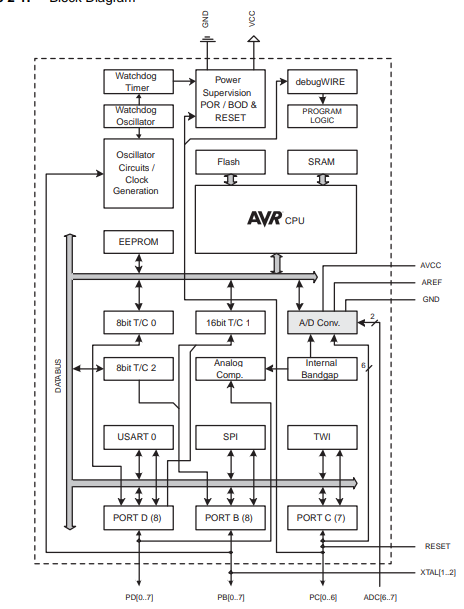
\includegraphics[width=.8\linewidth]{Imagenes/1.png}
 \caption{Diagrama de bloques de ATMega328P. Tomado de \cite{web1}.}
 \label{fig1}
\end{figure}

\begin{figure}[H]
\centering
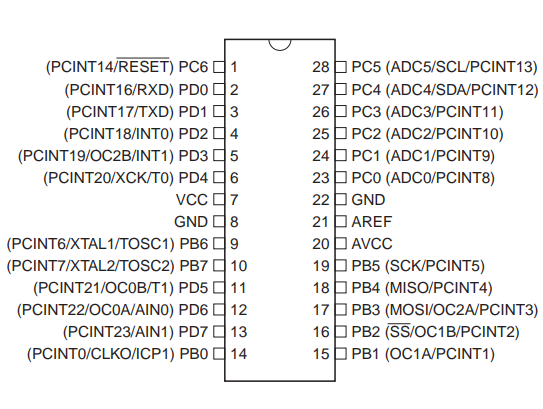
\includegraphics[width=.8\linewidth]{Imagenes/2.png}
 \caption{Diagrama de pines de ATMega328P. Tomado de \cite{web1}.}
 \label{fig2}
\end{figure}
Dado que será necesario saber a profundidad la clasificación de estos pines la figura \ref{fig2.1} brinda una mejor clasificación de éstos.
\begin{figure}[H]
\centering
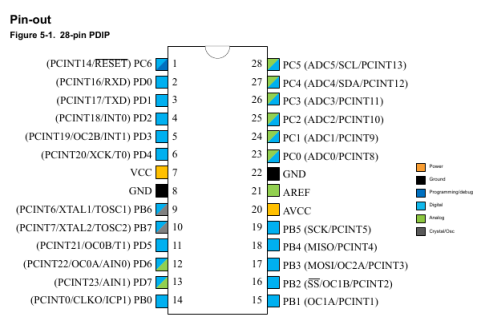
\includegraphics[width=.8\linewidth]{Imagenes/2.1.png}
 \caption{Clasificación de pines de ATMega328P. Tomado de \cite{web5}.}
 \label{fig2.1}
\end{figure}

\subsubsection*{Características eléctricas}
La siguiente lista describe estos detalles.
\begin{itemize}
\item Voltaje: 1.8-\SI{5.5}{\volt}.
\item Velocidad: 0-\SI{4}{\mega\Hz},  1.8-\SI{5.5}{\volt}. 0-\SI{10}{\mega\Hz},  2.7-\SI{5.5}{\volt}. 0-\SI{20}{\mega\Hz},  4.5-\SI{5.5}{\volt}
\item Modo activo: \SI{0.3}{\mA}
\item Temperatura de funcionamiento: $-55^\circ$ a +$125^\circ$.
\item Temperatura de almacenamiento: $-65^\circ$ a +$125^\circ$.
\item Temperatura pin RESET y GND: -\SI{0.5}{\volt} a \SI{13}{\volt}.
\item Temperatura en los demás pines: -\SI{0.5}{\volt} a VCC\SI{0.5}{\volt}.
\item Corriente por pin I/O: \SI{40}{\mA}.
\end{itemize}
Sabiendo lo anterior, resulta pertinente mencionar la descripción de los pines usados en este laboratorio. Para la conexión de las fuentes de DC y AC, se usaron los pines \texttt{A5, A4, A3, A2}. Que se caracterizan por ser entre analógicos y digitales, esto permite tener más facilidad en cuanto a funciones. Mismo escenario para el botón de modo AC, solo que en este caso está conectado al pin \texttt{A0}. En cuanto a los pines que activan las alarmas de los LEDs y los que se conectaron a la pantalla PCD8544 se han usado los que son totalmente digitales (11-3), es decir, estos pines solo pueden funcionar como salidas o entradas, por lo que se declaron como \texttt{INPUT} o \texttt{OUTPUT}. Por último, para la comunicación serial se usaron los pines \texttt{RX} y \texttt{TX}, ya que son los encargados de la comunicación.
\subsection*{Periféricos utilizados}
Algunos periféricos usados del microcontrolador así como la pantalla PCD8544 fueron los siguientes:
\begin{itemize}
\item \textbf{pinMode:} esto se usó para cual pin era una entrada o salida, y esto ayuda para que el microcontrolador entienda todas las acciones que se desea realizar.
\item \textbf{digitalWrite:} básicamente su función es para establecer el estado de una variable después de una acción, típicamente es para poner en alto o en bajo una señal.
\item \textbf{analogRead:} esto devuelve el valor leído del pin de entrada analógico, el valor es proporcional a la entrada analógica tomando como base una tensión de referencia: 0-1023.
\item \textbf{display.begin:} inicia/enciende la pantalla.
\item \textbf{display.setContrast:} configuración del contraste de la pantalla.
\item \textbf{display.clearDisplay:} limpia la pantalla.
\item \textbf{display.setTextSize:} configura la posición del texto.
\item \textbf{display.setTextColor:} establece el color de las letras.
\item \textbf{display.setCursor:} este parámetro sirve para posicionar el texto en la pantalla.
\item \textbf{display.println:} imprime el contenido deseado.
\item \textbf{display.display:} imprime el logo de Adafruit y se coloca después de cada texto, de lo contrario no se mostrará el contenido.
\end{itemize}
Si bien, se debe mencionar que la pantalla PCD8544 desempeña un papel importante en este trabajo, porque permite mostrar las magnitudes de las tensiones eléctricas en las fuentes de alimentación, tanto para modo DC como AC. Por tanto, hay que conocer los pines que se usaron para darle sentido a los pererféricos mencionados anteriormente. En el simulador se tienen 5 pines que se explican a continuación \cite{web2}.
\begin{itemize}
\item \textbf{RST:} esta señal reiniciará el dispositivo y debe ser aplicado adecuadamente al chip. La señal activa está en bajo.
\item \textbf{CS:} habilita la pantalla con el que se está comunicando en un bus SPI. Cuando esta señal está activa, el PCD8544 está habilitado y listo para recibir comandos o datos a través del bus SPI. Cuando la señal CS está inactiva, la pantalla no responde y no acepta datos.
\item \textbf{D/C:} selecciona el modo de operación, alto o bajo.
\item \textbf{DIN:} es una entrada para la línea de datos.
\item \textbf{CLK:} es la señal de reloj que va de 0.0 a 4.0 Mbit/s.
\end{itemize}
Por lo que, los datos que se muestran en la pantalla PCD8544 es porque se usa el modelo de comunicaciones SPI: \texttt{Serial Peripheral Interface}, es un bus de interfaz comúnmente utilizado para enviar datos entre microcontroladores y pequeños periféricos como registros de desplazamiento, sensores y tarjetas SD \cite{web3}.
\subsection*{Componentes electrónicos complementarios}
Algunos de los componentes extra que fueron de gran ayuda para el diseño del voltímetro fueron los siguientes:
\begin{itemize}
\item Amplificadores inversores: se optó por esta opción, ya que el voltaje de salida de este tipo de amplificadores tienen la siguiente expresión:
\begin{equation}
v_o=-v_i\cdot \frac{R_2}{R1}
\label{eq1}
\end{equation}
Esto sirvió para diseñar que los rangos de tensión eléctrica no fueron mayores a \SI{5}{\volt}. De esa manera, la base para lograr esto fue con valores de $R_1=R_2=\SI{2.5}{\ohm}$ y $v_i=\SI{-2.5}{\volt}$,
\begin{figure}[H]
\centering
 \begin{circuitikz} \draw
 (0,0) node[op amp] (opamp) {}
 (opamp.+) node[left] {} node[ground] {}
 (opamp.-) node[left] {}
 (opamp.-) node[left] {}
 (opamp.out) node[right] {$v_o$};
 %\draw (0,0)--(opamp.-);
 \draw (-3,0.5) to[R=$R_1$,-*](opamp.-);
 \draw (-4,0.5)node[above]{$v_i$} to [short, o-](-3,0.5);
 \draw (opamp.-)--(-1.2,2.2)to[R=$R_2$](1.1, 2.2)to[short, -*](1.1,0);
\end{circuitikz}
\caption{Amplificador inversor.}
 \label{ampOp}
\end{figure}

A partir, del esquemático anterior y la fórmula \ref{eq1} fue posible regular las fuentes de tensión AC/DC para los 4 canales con el objetivo de obtener las mejores aproximaciones con respecto al voltímetro y lo mostrado en la pantalla.
\item Relay: en este componente se conectan las 8 entradas de las fuentes AC/DC y salen 4 que están conectadas a los amplificadores inversores, la idea es determinar cuando las fuentes AC y DC estén normalmente cerradas o normalmente abiertas.
\item Switches: son de gran ayuda para definir en que estado opera el voltímetro, si está realizando mediciones en AC o en DC, para realizar correctas lecturas de este cambio se debe tener en cuenta el diseño previo de valores de resistencia y capacitancia para evitar falsas lecturas. 
\begin{figure}[H]
\centering
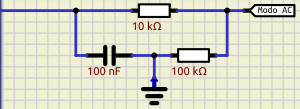
\includegraphics[width=.8\linewidth]{Imagenes/3.1.png}
 \caption{Diseño antirebote.}
 \label{fig3.1}
\end{figure}
El diseño anterior, ayuda a que la transición de DC a AC sea inmediata.
\end{itemize}

\subsection*{Lista de componentes}
La siguiente tabla resume los componentes (con sus precios) utilizados para este trabajo. La lista de precios mostrados en la tabla \ref{table_2} se tomaron de \cite{web4}. %FALTA AGREGAR LO RESTANTE DE LA COMUNICACION SERIAL.
\begin{table}[H]
\caption{Lista de equipos}
\label{table_2}
\begin{center}
\begin{tabular}{r|cc}
\hline
\textbf{Componente}&\textbf{Cantidad}&\textbf{Precio}\\
 \hline
Arduino UNO&1   &17\$ \\ \hline 
Kit de resistencias &1   &9.99\$ \\ \hline 
Capacitancias&1   &0.2\$ \\ \hline 
LEDs&4   &2.2\$ \\ \hline 
Pantalla PCD8544&1   &5.85\$ \\ \hline 
Botón&9   &5.85\$ \\ \hline 
Amplificadores&4   &3.8\$ \\ \hline 
RelaySPST & 2 & 29\$ \\ \hline 
Fuente de voltaje AC/DC& 1&48.95\$\\ \hline 

 \textbf{Total}& &  122.84\\
 \hline
\end{tabular}
\end{center}
\end{table}

\subsection*{Diseño del circuito}
El circuito que simula el voltímetro se muestra en la figura \ref{fig3}.
\begin{figure}[H]
\centering
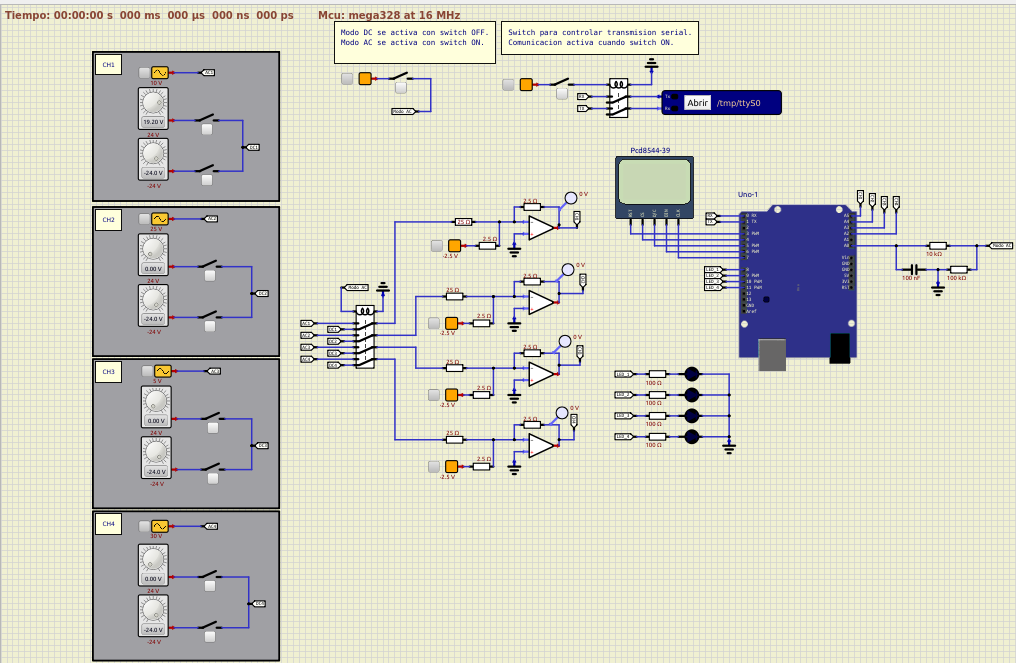
\includegraphics[width=.8\linewidth]{Imagenes/7.png}
 \caption{Circuito del voltímetro}
 \label{fig3}
\end{figure}
Inicialmente, se hizo uso del amplificador inversor para lograr obtener una magnitud de tensión eléctrica adecuada y así no sobrepasar el umbral del arduino. Tal como se mostró en la sección de componentes complementarios, tomar esos valores de resistencias y elegir un voltaje de magnitud negativa dará un valor adecuado que permita colocar fuentes de tensión para el buen funcionamiento del voltímetro. 
\begin{figure}[H]
\centering
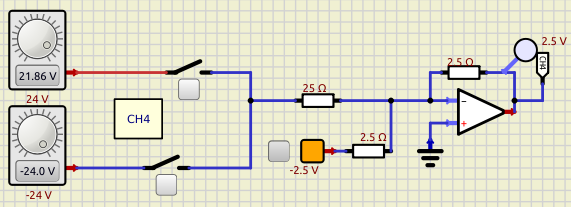
\includegraphics[width=.8\linewidth]{Imagenes/4.png}
 \caption{Tensión de salida a medir.}
 \label{fig4}
\end{figure}
Esto se realizó para los 4 canales que se van usar, los cuales se conectaron como entradas al arduino en los pines \texttt{A5-A2}. Luego, en los pines 7-3 se conectaron las señales \texttt{CLK, DIN, D/C, CS, RST} respectivamente, esto para realizar unas pequeñas pruebas de funcionamiento de la pantalla mostrando un pequeño mensaje para comprobar su correcta conexión. En la sección de resultados se darán más detalles de este diseño.
\begin{figure}[H]
\centering
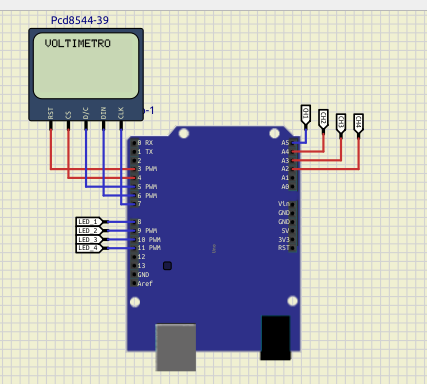
\includegraphics[width=.8\linewidth]{Imagenes/5.png}
 \caption{Funcionamiento correcto de la pantalla PCD8544.}
 \label{fig5}
\end{figure}
Después, la conexión de los LEDs de alarma al arduino en los pines 8-11 que fueron configurados como salidas, se van a encender cuando se supere el rango de -20 a 20 en DC, y -14.14 a 14.14 en AC.
\begin{figure}[H]
\centering
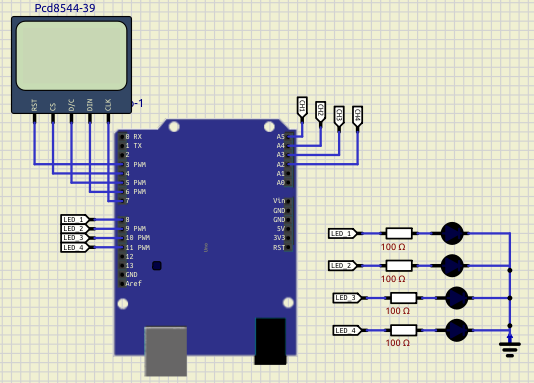
\includegraphics[width=.8\linewidth]{Imagenes/6.png}
 \caption{Conexión de los LEDs al arduino.}
 \label{fig6}
\end{figure}
Otro detalle, para ordenar el voltímetro se decidió usar un relay que sirve de puente entre las fuentes AC/DC y la salida de los amplificadores inversores que se comunicará con la PCD8544, la cual mostrará las tensiones eléctricas en AC (si el botón está en alto) o en DC, enviará señales a los LEDS y estos se pondrán en alto o no dependiendo de las magnitudes que tengan las fuentes variables de tensión y reflejadas en la PCD8544. Esto se ve de la siguiente manera \footnote{Por resolución de la imagen solo se mostrarán 3, en realidad posee 4.}.
\begin{figure}[H]
\centering
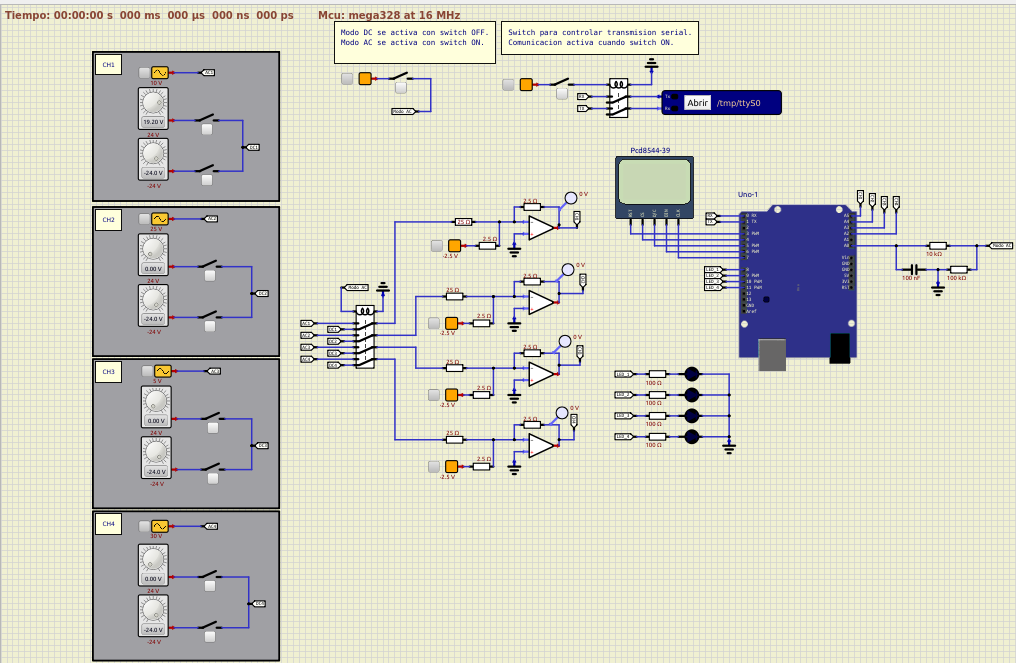
\includegraphics[width=.8\linewidth]{Imagenes/7.png}
 \caption{Canales del voltímetro.}
 \label{fig7}
\end{figure}
Ahora, para la comunicación serial se introduce un puerto serial encargado de realizar la comunicación entre el arduino y el puerto serial, también se hace uso de un relé para hacer cumplir con lo solicitado de que la transmisión se pueda controlar por medio de un switch, el resultado final se observa en la siguiente figura:
\begin{figure}[H]
    \centering
    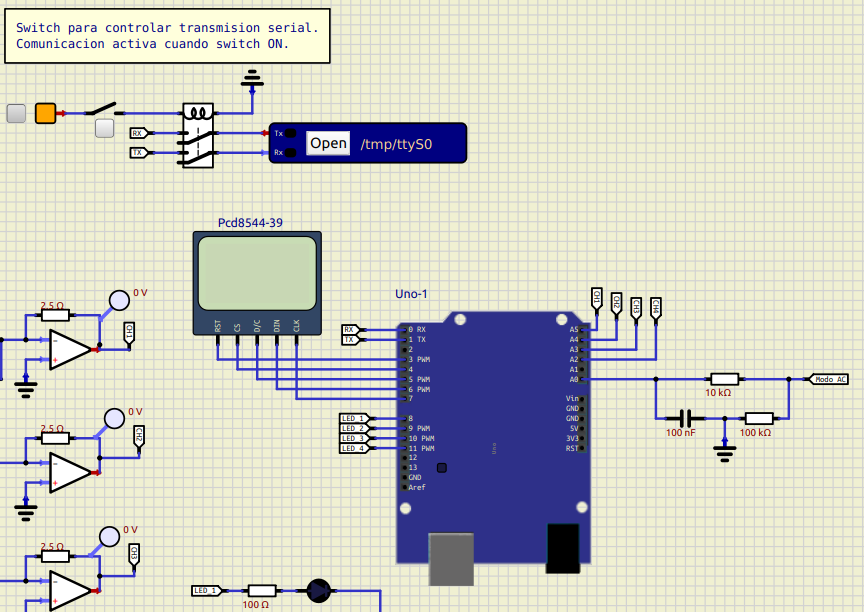
\includegraphics[width=.8\linewidth]{Imagenes/8.png}
    \caption{Introducción del puerto serial y el switch para realizar la comunicación.}
    \label{figk1}
\end{figure}

Es importante cuando se hace la conexión ver que se toma el RX de un puerto y se conecta con el puerto TX para que se pueda dar la comunicación como se vio en clases.
\newpage


\section{Desarrollo/Análisis}
El diagrama de bloques generales para el funcionamiento del voltímetro es el siguiente.
\begin{figure}[H]

\centering
\tikzset{every picture/.style={line width=0.75pt}} %set default line width to 0.75pt        

\begin{tikzpicture}[x=0.75pt,y=0.75pt,yscale=-1,xscale=1]
%uncomment if require: \path (0,736); %set diagram left start at 0, and has height of 736

%Flowchart: Connector [id:dp7813495520702245] 
\draw   (320,81) .. controls (320,66.64) and (331.64,55) .. (346,55) .. controls (360.36,55) and (372,66.64) .. (372,81) .. controls (372,95.36) and (360.36,107) .. (346,107) .. controls (331.64,107) and (320,95.36) .. (320,81) -- cycle ;
%Straight Lines [id:da8847526091998554] 
\draw    (345.92,107) -- (345.92,123) ;
\draw [shift={(345.92,126)}, rotate = 270] [fill={rgb, 255:red, 0; green, 0; blue, 0 }  ][line width=0.08]  [draw opacity=0] (8.93,-4.29) -- (0,0) -- (8.93,4.29) -- cycle    ;
%Flowchart: Process [id:dp3892985602062795] 
\draw   (285,127) -- (407,127) -- (407,160) -- (285,160) -- cycle ;
%Flowchart: Decision [id:dp21596588394867888] 
\draw   (347.92,180) -- (419.9,235.5) -- (347.92,291) -- (275.94,235.5) -- cycle ;
%Straight Lines [id:da7204417446380422] 
\draw    (347.92,161) -- (347.92,177) ;
\draw [shift={(347.92,180)}, rotate = 270] [fill={rgb, 255:red, 0; green, 0; blue, 0 }  ][line width=0.08]  [draw opacity=0] (8.93,-4.29) -- (0,0) -- (8.93,4.29) -- cycle    ;
%Straight Lines [id:da451260237829443] 
\draw    (489,256) -- (489,272) ;
\draw [shift={(489,275)}, rotate = 270] [fill={rgb, 255:red, 0; green, 0; blue, 0 }  ][line width=0.08]  [draw opacity=0] (8.93,-4.29) -- (0,0) -- (8.93,4.29) -- cycle    ;
%Straight Lines [id:da49582350632228556] 
\draw    (225,256) -- (225,272) ;
\draw [shift={(225,275)}, rotate = 270] [fill={rgb, 255:red, 0; green, 0; blue, 0 }  ][line width=0.08]  [draw opacity=0] (8.93,-4.29) -- (0,0) -- (8.93,4.29) -- cycle    ;
%Straight Lines [id:da9013438330772021] 
\draw    (153.04,507) -- (190,506.08) ;
\draw [shift={(193,506)}, rotate = 178.57] [fill={rgb, 255:red, 0; green, 0; blue, 0 }  ][line width=0.08]  [draw opacity=0] (8.93,-4.29) -- (0,0) -- (8.93,4.29) -- cycle    ;
%Straight Lines [id:da797473974800426] 
\draw    (330,505) -- (270,505) ;
\draw [shift={(267,505)}, rotate = 360] [fill={rgb, 255:red, 0; green, 0; blue, 0 }  ][line width=0.08]  [draw opacity=0] (8.93,-4.29) -- (0,0) -- (8.93,4.29) -- cycle    ;
%Straight Lines [id:da006314317293441896] 
\draw    (232,531) -- (232,547) ;
\draw [shift={(232,550)}, rotate = 270] [fill={rgb, 255:red, 0; green, 0; blue, 0 }  ][line width=0.08]  [draw opacity=0] (8.93,-4.29) -- (0,0) -- (8.93,4.29) -- cycle    ;
%Straight Lines [id:da9058055932314646] 
\draw    (303.98,605.5) -- (351,605.03) ;
\draw [shift={(354,605)}, rotate = 179.43] [fill={rgb, 255:red, 0; green, 0; blue, 0 }  ][line width=0.08]  [draw opacity=0] (8.93,-4.29) -- (0,0) -- (8.93,4.29) -- cycle    ;
%Straight Lines [id:da1932315478192832] 
\draw    (489.92,306) -- (489.92,322) ;
\draw [shift={(489.92,325)}, rotate = 270] [fill={rgb, 255:red, 0; green, 0; blue, 0 }  ][line width=0.08]  [draw opacity=0] (8.93,-4.29) -- (0,0) -- (8.93,4.29) -- cycle    ;
%Straight Lines [id:da6050013822698619] 
\draw    (20,138) -- (271,138) ;
\draw [shift={(274,138)}, rotate = 180] [fill={rgb, 255:red, 0; green, 0; blue, 0 }  ][line width=0.08]  [draw opacity=0] (8.93,-4.29) -- (0,0) -- (8.93,4.29) -- cycle    ;
%Shape: Right Angle [id:dp24954692627046726] 
\draw   (419.9,235.5) -- (489,235.5) -- (489,256) ;
%Flowchart: Process [id:dp33592140600780107] 
\draw   (428,276) -- (557,276) -- (557,306) -- (428,306) -- cycle ;
%Shape: Right Angle [id:dp2914826540765745] 
\draw   (275.94,235.5) -- (225,235.5) -- (225,256) ;
%Flowchart: Decision [id:dp9064156706798434] 
\draw   (225,275) -- (296.98,330.5) -- (225,386) -- (153.02,330.5) -- cycle ;
%Straight Lines [id:da6126735924115385] 
\draw    (341,351) -- (341,367) ;
\draw [shift={(341,370)}, rotate = 270] [fill={rgb, 255:red, 0; green, 0; blue, 0 }  ][line width=0.08]  [draw opacity=0] (8.93,-4.29) -- (0,0) -- (8.93,4.29) -- cycle    ;
%Shape: Right Angle [id:dp7943090498770735] 
\draw   (296.98,330.5) -- (341,330.5) -- (341,351) ;
%Straight Lines [id:da7128924347373624] 
\draw    (105,352) -- (105,368) ;
\draw [shift={(105,371)}, rotate = 270] [fill={rgb, 255:red, 0; green, 0; blue, 0 }  ][line width=0.08]  [draw opacity=0] (8.93,-4.29) -- (0,0) -- (8.93,4.29) -- cycle    ;
%Shape: Right Angle [id:dp8866366667209189] 
\draw   (155.94,331.5) -- (105,331.5) -- (105,352) ;
%Flowchart: Process [id:dp15212318966923655] 
\draw   (32,372) -- (177,372) -- (177,420) -- (32,420) -- cycle ;
%Flowchart: Process [id:dp5589357347254946] 
\draw   (268,370) -- (413,370) -- (413,418) -- (268,418) -- cycle ;
%Shape: Right Angle [id:dp26602461789391585] 
\draw   (153.04,507) -- (106.94,507) -- (106.94,420.5) ;
%Shape: Right Angle [id:dp9899984887472151] 
\draw   (330,505) -- (344.94,505) -- (344.94,419.5) ;
%Flowchart: Decision [id:dp9568469291538075] 
\draw   (232,550) -- (303.98,605.5) -- (232,661) -- (160.02,605.5) -- cycle ;
%Flowchart: Connector [id:dp7268194319410761] 
\draw   (206,505) .. controls (206,490.64) and (217.64,479) .. (232,479) .. controls (246.36,479) and (258,490.64) .. (258,505) .. controls (258,519.36) and (246.36,531) .. (232,531) .. controls (217.64,531) and (206,519.36) .. (206,505) -- cycle ;
%Flowchart: Process [id:dp8372151895077977] 
\draw   (354,581) -- (428,581) -- (428,624) -- (354,624) -- cycle ;
%Shape: Right Angle [id:dp04700865884221406] 
\draw   (160.02,605.5) -- (20,605.5) -- (20,138) ;
%Shape: Right Angle [id:dp6697593994914697] 
\draw   (112,682) -- (388.94,682) -- (388.94,624.5) ;
%Straight Lines [id:da9427664494344408] 
\draw    (112,682) -- (112,616) ;
\draw [shift={(112,613)}, rotate = 90] [fill={rgb, 255:red, 0; green, 0; blue, 0 }  ][line width=0.08]  [draw opacity=0] (8.93,-4.29) -- (0,0) -- (8.93,4.29) -- cycle    ;
%Flowchart: Process [id:dp6713652946060731] 
\draw   (426,324) -- (555,324) -- (555,354) -- (426,354) -- cycle ;

% Text Node
\draw (329,71) node [anchor=north west][inner sep=0.75pt]   [align=left] {Inicio};
% Text Node
\draw (292,134) node [anchor=north west][inner sep=0.75pt]   [align=left] {Enviar tensiones};
% Text Node
\draw (301,213) node [anchor=north west][inner sep=0.75pt]   [align=left] {Pantalla ON\\ serial abierta ON?};
% Text Node
\draw (430,280) node [anchor=north west][inner sep=0.75pt]   [align=left] {Comunicación PC};
% Text Node
\draw (182,314) node [anchor=north west][inner sep=0.75pt]   [align=left] {switch AC/DC\\ abierto ?};
% Text Node
\draw (287,374) node [anchor=north west][inner sep=0.75pt]   [align=left] {Calcular, enviar\\DC valores};
% Text Node
\draw (169,595) node [anchor=north west][inner sep=0.75pt]   [align=left] {20V$\displaystyle < $val $\displaystyle < $-20V};
% Text Node
\draw (363,595) node [anchor=north west][inner sep=0.75pt]   [align=left] {LED ON};
% Text Node
\draw (468,215) node [anchor=north west][inner sep=0.75pt]   [align=left] {No};
% Text Node
\draw (217,211) node [anchor=north west][inner sep=0.75pt]   [align=left] {Si};
% Text Node
\draw (326,311) node [anchor=north west][inner sep=0.75pt]   [align=left] {No};
% Text Node
\draw (97,307) node [anchor=north west][inner sep=0.75pt]   [align=left] {Si};
% Text Node
\draw (60,378) node [anchor=north west][inner sep=0.75pt]   [align=left] {Calcular, enviar\\AC valores};
% Text Node
\draw (326,584) node [anchor=north west][inner sep=0.75pt]   [align=left] {Si};
% Text Node
\draw (133,584) node [anchor=north west][inner sep=0.75pt]   [align=left] {No};
% Text Node
\draw (445,329) node [anchor=north west][inner sep=0.75pt]   [align=left] {Creación csv};


\end{tikzpicture}
\caption{Diagrama de bloques general}
\label{dia_General}
\end{figure}
Una vez que se activen alguna de las fuentes, en la pantalla PCD8544 se mostrará las magnitudes (despreciables, \SI{0.05}{\volt}) por default en cada canal, y al estar el botón de modo AC/DC en bajo por tanto, en esta pantalla se mostrarán los valores en DC, si éste se pone en alto entonces en la pantalla se mostrarán los valores rms en AC, ahora, dependiendo de las magnitudes que se ajusten en ambos modos los LEDs de alarma se encenderán o no, que al mismo tiempo se verán en la pantalla. Por último, al presionar el botón de comunicación serial, se establece la comunicación adecuada para generar el informe del archivo csv.\par
Luego, para realizar las medidas adecuadas se tuvo que realizar una función capaz de normalizar y escalar en el intervalo de rango solicitado: [-24, 24]. 
\begin{figure}[H]
\centering


\tikzset{every picture/.style={line width=0.75pt}} %set default line width to 0.75pt        

\begin{tikzpicture}[x=0.75pt,y=0.75pt,yscale=-1,xscale=1]
%uncomment if require: \path (0,491); %set diagram left start at 0, and has height of 491

%Flowchart: Connector [id:dp7813495520702245] 
\draw   (320,81) .. controls (320,66.64) and (331.64,55) .. (346,55) .. controls (360.36,55) and (372,66.64) .. (372,81) .. controls (372,95.36) and (360.36,107) .. (346,107) .. controls (331.64,107) and (320,95.36) .. (320,81) -- cycle ;
%Straight Lines [id:da8847526091998554] 
\draw    (345.92,107) -- (345.92,123) ;
\draw [shift={(345.92,126)}, rotate = 270] [fill={rgb, 255:red, 0; green, 0; blue, 0 }  ][line width=0.08]  [draw opacity=0] (8.93,-4.29) -- (0,0) -- (8.93,4.29) -- cycle    ;
%Flowchart: Process [id:dp3892985602062795] 
\draw   (285,127) -- (407,127) -- (407,160) -- (285,160) -- cycle ;
%Flowchart: Decision [id:dp21596588394867888] 
\draw   (347.92,180) -- (388.45,212.5) -- (347.92,245) -- (307.39,212.5) -- cycle ;
%Straight Lines [id:da7204417446380422] 
\draw    (347.92,161) -- (347.92,177) ;
\draw [shift={(347.92,180)}, rotate = 270] [fill={rgb, 255:red, 0; green, 0; blue, 0 }  ][line width=0.08]  [draw opacity=0] (8.93,-4.29) -- (0,0) -- (8.93,4.29) -- cycle    ;
%Straight Lines [id:da451260237829443] 
\draw    (457.55,233) -- (457.55,249) ;
\draw [shift={(457.55,252)}, rotate = 270] [fill={rgb, 255:red, 0; green, 0; blue, 0 }  ][line width=0.08]  [draw opacity=0] (8.93,-4.29) -- (0,0) -- (8.93,4.29) -- cycle    ;
%Straight Lines [id:da49582350632228556] 
\draw    (256.45,233) -- (256.45,249) ;
\draw [shift={(256.45,252)}, rotate = 270] [fill={rgb, 255:red, 0; green, 0; blue, 0 }  ][line width=0.08]  [draw opacity=0] (8.93,-4.29) -- (0,0) -- (8.93,4.29) -- cycle    ;
%Straight Lines [id:da006314317293441896] 
\draw    (327,351) -- (327,367) ;
\draw [shift={(327,348)}, rotate = 90] [fill={rgb, 255:red, 0; green, 0; blue, 0 }  ][line width=0.08]  [draw opacity=0] (8.93,-4.29) -- (0,0) -- (8.93,4.29) -- cycle    ;
%Straight Lines [id:da6050013822698619] 
\draw    (356,166.02) -- (540,167) ;
\draw [shift={(353,166)}, rotate = 0.31] [fill={rgb, 255:red, 0; green, 0; blue, 0 }  ][line width=0.08]  [draw opacity=0] (8.93,-4.29) -- (0,0) -- (8.93,4.29) -- cycle    ;
%Shape: Right Angle [id:dp24954692627046726] 
\draw   (388.45,212.5) -- (457.55,212.5) -- (457.55,233) ;
%Shape: Right Angle [id:dp2914826540765745] 
\draw   (307.39,212.5) -- (256.45,212.5) -- (256.45,233) ;
%Flowchart: Decision [id:dp9064156706798434] 
\draw   (256.92,305) -- (309.92,345.5) -- (256.92,386) -- (203.92,345.5) -- cycle ;
%Straight Lines [id:da6126735924115385] 
\draw    (457,283) -- (457,299) ;
\draw [shift={(457,302)}, rotate = 270] [fill={rgb, 255:red, 0; green, 0; blue, 0 }  ][line width=0.08]  [draw opacity=0] (8.93,-4.29) -- (0,0) -- (8.93,4.29) -- cycle    ;
%Shape: Right Angle [id:dp7943090498770735] 
\draw   (307.98,344.5) -- (540,344.5) -- (540,167) ;
%Straight Lines [id:da7128924347373624] 
\draw    (152.98,366) -- (152.98,382) ;
\draw [shift={(152.98,385)}, rotate = 270] [fill={rgb, 255:red, 0; green, 0; blue, 0 }  ][line width=0.08]  [draw opacity=0] (8.93,-4.29) -- (0,0) -- (8.93,4.29) -- cycle    ;
%Shape: Right Angle [id:dp8866366667209189] 
\draw   (203.92,345.5) -- (152.98,345.5) -- (152.98,366) ;
%Flowchart: Process [id:dp15212318966923655] 
\draw   (105,385) -- (201,385) -- (201,422) -- (105,422) -- cycle ;
%Shape: Right Angle [id:dp9899984887472151] 
\draw   (199,460) -- (327,460) -- (327,367) ;
%Flowchart: Connector [id:dp7268194319410761] 
\draw   (437,320.5) .. controls (437,310.28) and (445.95,302) .. (457,302) .. controls (468.05,302) and (477,310.28) .. (477,320.5) .. controls (477,330.72) and (468.05,339) .. (457,339) .. controls (445.95,339) and (437,330.72) .. (437,320.5) -- cycle ;
%Flowchart: Process [id:dp6713652946060731] 
\draw   (394,252) -- (523,252) -- (523,282) -- (394,282) -- cycle ;
%Straight Lines [id:da15691850789793538] 
\draw    (347.92,245) -- (347.92,261) ;
\draw [shift={(347.92,264)}, rotate = 270] [fill={rgb, 255:red, 0; green, 0; blue, 0 }  ][line width=0.08]  [draw opacity=0] (8.93,-4.29) -- (0,0) -- (8.93,4.29) -- cycle    ;
%Flowchart: Process [id:dp025828036440153967] 
\draw   (189,253) -- (324,253) -- (324,286) -- (189,286) -- cycle ;
%Straight Lines [id:da2671209465635622] 
\draw    (256.92,286) -- (256.92,302) ;
\draw [shift={(256.92,305)}, rotate = 270] [fill={rgb, 255:red, 0; green, 0; blue, 0 }  ][line width=0.08]  [draw opacity=0] (8.93,-4.29) -- (0,0) -- (8.93,4.29) -- cycle    ;
%Straight Lines [id:da2035552754915979] 
\draw    (150,422) -- (150,438) ;
\draw [shift={(150,441)}, rotate = 270] [fill={rgb, 255:red, 0; green, 0; blue, 0 }  ][line width=0.08]  [draw opacity=0] (8.93,-4.29) -- (0,0) -- (8.93,4.29) -- cycle    ;
%Flowchart: Process [id:dp8396019792624998] 
\draw   (101,441) -- (197,441) -- (197,478) -- (101,478) -- cycle ;

% Text Node
\draw (329,71) node [anchor=north west][inner sep=0.75pt]   [align=left] {Inicio};
% Text Node
\draw (306,134) node [anchor=north west][inner sep=0.75pt]   [align=left] {max\_val = 0};
% Text Node
\draw (327,205) node [anchor=north west][inner sep=0.75pt]   [align=left] {i$<$100};
% Text Node
\draw (215,336) node [anchor=north west][inner sep=0.75pt]   [align=left] {val$>$max\_val};
% Text Node
\draw (438,193) node [anchor=north west][inner sep=0.75pt]   [align=left] {No};
% Text Node
\draw (248,194) node [anchor=north west][inner sep=0.75pt]   [align=left] {Si};
% Text Node
\draw (337,325) node [anchor=north west][inner sep=0.75pt]   [align=left] {No};
% Text Node
\draw (147,328) node [anchor=north west][inner sep=0.75pt]   [align=left] {Si};
% Text Node
\draw (106.12,395) node [anchor=north west][inner sep=0.75pt]   [align=left] {val = max\_val};
% Text Node
\draw (413,257) node [anchor=north west][inner sep=0.75pt]   [align=left] {return max\_val};
% Text Node
\draw (196,260) node [anchor=north west][inner sep=0.75pt]   [align=left] {analogRead(mag)};
% Text Node
\draw (126.12,451) node [anchor=north west][inner sep=0.75pt]   [align=left] {delay()};
% Text Node
\draw (448,310) node [anchor=north west][inner sep=0.75pt]   [align=left] {fin};


\end{tikzpicture}
\caption{Diagrama de flujo función mide\_voltaje}
\label{sch3}
\end{figure}
Esta función se compone de un ciclo \texttt{for} que va iterando los valores que poseen los 4 canales y realiza una resta de 511 (la mitad de 1023) y voltaje medido, luego se hace la escala con el producto de esta substacción y la división de 48 entre 1023, todo esto para lograr manipular voltajes de \SI{0}{\volt}-\SI{5}{\volt} con el objetivo de normalizar y escalar el valor máximo medido.\par
La función para generar las alarmas tanto en DC como en AC son muy similares, por lo que el siguiente diagrama de bloques es equivalente para ambos.
\begin{figure}[H]
\centering


\tikzset{every picture/.style={line width=0.75pt}} %set default line width to 0.75pt        

\begin{tikzpicture}[x=0.75pt,y=0.75pt,yscale=-1,xscale=1]
%uncomment if require: \path (0,689); %set diagram left start at 0, and has height of 689

%Flowchart: Connector [id:dp7813495520702245] 
\draw   (315,40) .. controls (315,25.64) and (326.64,14) .. (341,14) .. controls (355.36,14) and (367,25.64) .. (367,40) .. controls (367,54.36) and (355.36,66) .. (341,66) .. controls (326.64,66) and (315,54.36) .. (315,40) -- cycle ;
%Straight Lines [id:da8847526091998554] 
\draw    (339.92,67) -- (339.92,83) ;
\draw [shift={(339.92,86)}, rotate = 270] [fill={rgb, 255:red, 0; green, 0; blue, 0 }  ][line width=0.08]  [draw opacity=0] (8.93,-4.29) -- (0,0) -- (8.93,4.29) -- cycle    ;
%Flowchart: Decision [id:dp21596588394867888] 
\draw   (341.35,135) -- (418,193.5) -- (341.35,252) -- (264.69,193.5) -- cycle ;
%Straight Lines [id:da7204417446380422] 
\draw    (341.35,116) -- (341.35,132) ;
\draw [shift={(341.35,135)}, rotate = 270] [fill={rgb, 255:red, 0; green, 0; blue, 0 }  ][line width=0.08]  [draw opacity=0] (8.93,-4.29) -- (0,0) -- (8.93,4.29) -- cycle    ;
%Straight Lines [id:da49582350632228556] 
\draw    (213.76,214) -- (213.76,230) ;
\draw [shift={(213.76,233)}, rotate = 270] [fill={rgb, 255:red, 0; green, 0; blue, 0 }  ][line width=0.08]  [draw opacity=0] (8.93,-4.29) -- (0,0) -- (8.93,4.29) -- cycle    ;
%Straight Lines [id:da6050013822698619] 
\draw    (138,101) -- (289,101.98) ;
\draw [shift={(292,102)}, rotate = 180.37] [fill={rgb, 255:red, 0; green, 0; blue, 0 }  ][line width=0.08]  [draw opacity=0] (8.93,-4.29) -- (0,0) -- (8.93,4.29) -- cycle    ;
%Shape: Right Angle [id:dp2914826540765745] 
\draw   (264.69,193.5) -- (213.76,193.5) -- (213.76,214) ;
%Shape: Right Angle [id:dp7943090498770735] 
\draw   (142.92,544) -- (138,544) -- (138,101) ;
%Straight Lines [id:da15691850789793538] 
\draw    (162,246) -- (142.91,246.86) ;
\draw [shift={(139.92,247)}, rotate = 357.41] [fill={rgb, 255:red, 0; green, 0; blue, 0 }  ][line width=0.08]  [draw opacity=0] (8.93,-4.29) -- (0,0) -- (8.93,4.29) -- cycle    ;
%Flowchart: Process [id:dp025828036440153967] 
\draw   (163,233) -- (275,233) -- (275,263) -- (163,263) -- cycle ;
%Flowchart: Process [id:dp08317044111396199] 
\draw   (294,87) -- (400,87) -- (400,115) -- (294,115) -- cycle ;
%Flowchart: Decision [id:dp9588588712187942] 
\draw   (341.35,271) -- (418,329.5) -- (341.35,388) -- (264.69,329.5) -- cycle ;
%Straight Lines [id:da6075623967992321] 
\draw    (341.35,252) -- (341.35,268) ;
\draw [shift={(341.35,271)}, rotate = 270] [fill={rgb, 255:red, 0; green, 0; blue, 0 }  ][line width=0.08]  [draw opacity=0] (8.93,-4.29) -- (0,0) -- (8.93,4.29) -- cycle    ;
%Straight Lines [id:da7280821078053175] 
\draw    (213.76,350) -- (213.76,366) ;
\draw [shift={(213.76,369)}, rotate = 270] [fill={rgb, 255:red, 0; green, 0; blue, 0 }  ][line width=0.08]  [draw opacity=0] (8.93,-4.29) -- (0,0) -- (8.93,4.29) -- cycle    ;
%Shape: Right Angle [id:dp5301940302382446] 
\draw   (264.69,329.5) -- (213.76,329.5) -- (213.76,350) ;
%Flowchart: Process [id:dp03155186296961898] 
\draw   (165,369) -- (280,369) -- (280,396) -- (165,396) -- cycle ;
%Straight Lines [id:da8674623880313952] 
\draw    (164,381) -- (144.91,381.86) ;
\draw [shift={(141.92,382)}, rotate = 357.41] [fill={rgb, 255:red, 0; green, 0; blue, 0 }  ][line width=0.08]  [draw opacity=0] (8.93,-4.29) -- (0,0) -- (8.93,4.29) -- cycle    ;
%Flowchart: Decision [id:dp9506954994828107] 
\draw   (341.35,417) -- (418,475.5) -- (341.35,534) -- (264.69,475.5) -- cycle ;
%Straight Lines [id:da2567401210333511] 
\draw    (213.76,496) -- (214.67,528) ;
\draw [shift={(214.76,531)}, rotate = 268.36] [fill={rgb, 255:red, 0; green, 0; blue, 0 }  ][line width=0.08]  [draw opacity=0] (8.93,-4.29) -- (0,0) -- (8.93,4.29) -- cycle    ;
%Shape: Right Angle [id:dp7317557872750253] 
\draw   (264.69,475.5) -- (213.76,475.5) -- (213.76,496) ;
%Flowchart: Process [id:dp6148244624650872] 
\draw   (166,531) -- (283,531) -- (283,560) -- (166,560) -- cycle ;
%Straight Lines [id:da6248486907124713] 
\draw    (165,543) -- (145.91,543.86) ;
\draw [shift={(142.92,544)}, rotate = 357.41] [fill={rgb, 255:red, 0; green, 0; blue, 0 }  ][line width=0.08]  [draw opacity=0] (8.93,-4.29) -- (0,0) -- (8.93,4.29) -- cycle    ;
%Straight Lines [id:da1967066179049608] 
\draw    (341.35,534) -- (341.35,550) ;
\draw [shift={(341.35,553)}, rotate = 270] [fill={rgb, 255:red, 0; green, 0; blue, 0 }  ][line width=0.08]  [draw opacity=0] (8.93,-4.29) -- (0,0) -- (8.93,4.29) -- cycle    ;
%Shape: Circle [id:dp6512187196885593] 
\draw   (316.35,578) .. controls (316.35,564.19) and (327.54,553) .. (341.35,553) .. controls (355.15,553) and (366.35,564.19) .. (366.35,578) .. controls (366.35,591.81) and (355.15,603) .. (341.35,603) .. controls (327.54,603) and (316.35,591.81) .. (316.35,578) -- cycle ;

% Text Node
\draw (324,30) node [anchor=north west][inner sep=0.75pt]   [align=left] {Inicio};
% Text Node
\draw (291,172) node [anchor=north west][inner sep=0.75pt]   [align=left] {$\displaystyle -20\geqslant $med\_1 \\$\displaystyle ||$ med\_1 $\displaystyle \geqslant 20$};
% Text Node
\draw (308,249) node [anchor=north west][inner sep=0.75pt]   [align=left] {No};
% Text Node
\draw (205,174) node [anchor=north west][inner sep=0.75pt]   [align=left] {Si};
% Text Node
\draw (177,240) node [anchor=north west][inner sep=0.75pt]   [align=left] {LED\_1 = ON};
% Text Node
\draw (303,93) node [anchor=north west][inner sep=0.75pt]   [align=left] {LEDs = OFF};
% Text Node
\draw (290,307) node [anchor=north west][inner sep=0.75pt]   [align=left] {$\displaystyle -20\geqslant $med\_2 \\$\displaystyle ||$ med\_2 $\displaystyle \geqslant 20$};
% Text Node
\draw (207,310) node [anchor=north west][inner sep=0.75pt]   [align=left] {Si};
% Text Node
\draw (176,374) node [anchor=north west][inner sep=0.75pt]   [align=left] {LED\_2 = ON};
% Text Node
\draw (338,384.4) node [anchor=north west][inner sep=0.75pt]  [font=\LARGE]  {$\vdots $};
% Text Node
\draw (334,569) node [anchor=north west][inner sep=0.75pt]   [align=left] {fin};
% Text Node
\draw (290,451) node [anchor=north west][inner sep=0.75pt]   [align=left] {$\displaystyle -20\geqslant $med\_4 \\$\displaystyle ||$ med\_4 $\displaystyle \geqslant 20$};
% Text Node
\draw (209,455) node [anchor=north west][inner sep=0.75pt]   [align=left] {Si};
% Text Node
\draw (182,536) node [anchor=north west][inner sep=0.75pt]   [align=left] {LED\_4 = ON};
% Text Node
\draw (314,395) node [anchor=north west][inner sep=0.75pt]   [align=left] {No};
% Text Node
\draw (314,525) node [anchor=north west][inner sep=0.75pt]   [align=left] {No};


\end{tikzpicture}

\caption{Diagrama de flujo alarma AC/DC.}
\label{sch4}
\end{figure}
Hasta este punto es posible mostrar el correcto funcionamiento del voltímetro con todos sus componentes. Primero se comprueba la medición de voltajes en DC.
\begin{figure}[H]
    \centering
    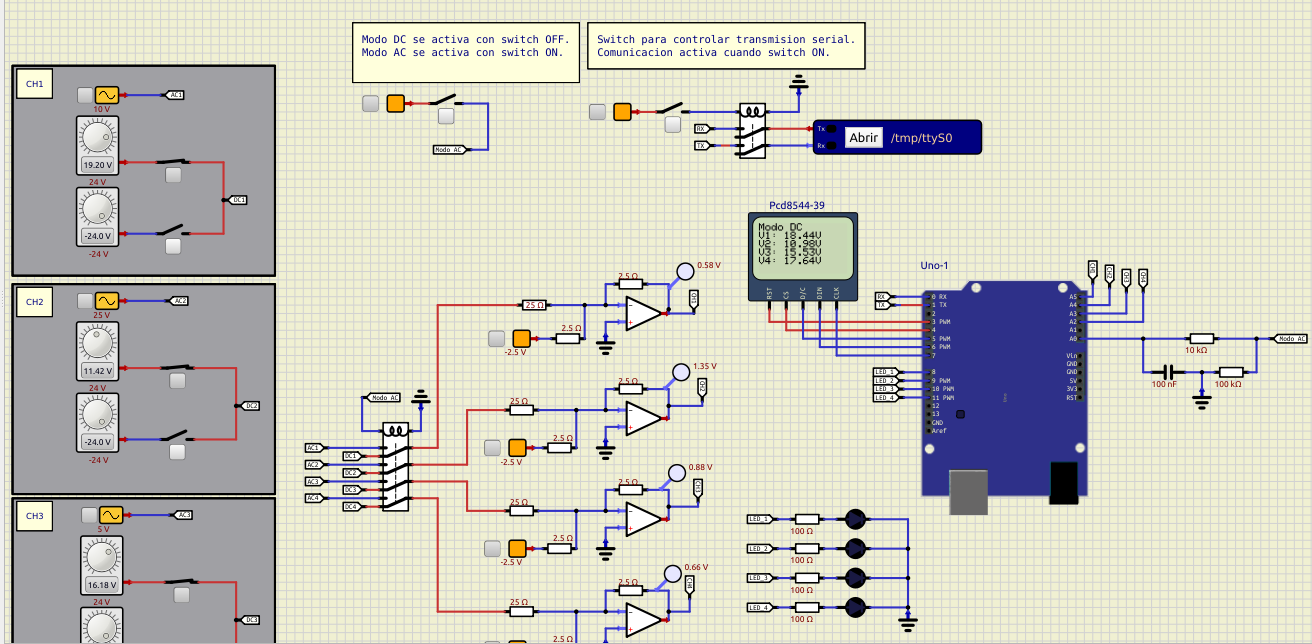
\includegraphics[width=.8\linewidth]{Imagenes/9.png}
    \caption{Medición de tensión DC de los 4 canales.}
    \label{fig_9}
\end{figure}
Se puede observar que la pantalla muestra las tensiones eléctricas en DC correctamente, es decir, el voltímetro es capaz de medir cuatro canales apropiadamente. Si se deseara ver la activación de los LEDs cuando se superan los umbrales de [-20, 20] basta con cambiar esto desde las fuentes. En la figura \ref{fig_10} se demuestra el resultado esperado.
\begin{figure}[H]
    \centering
    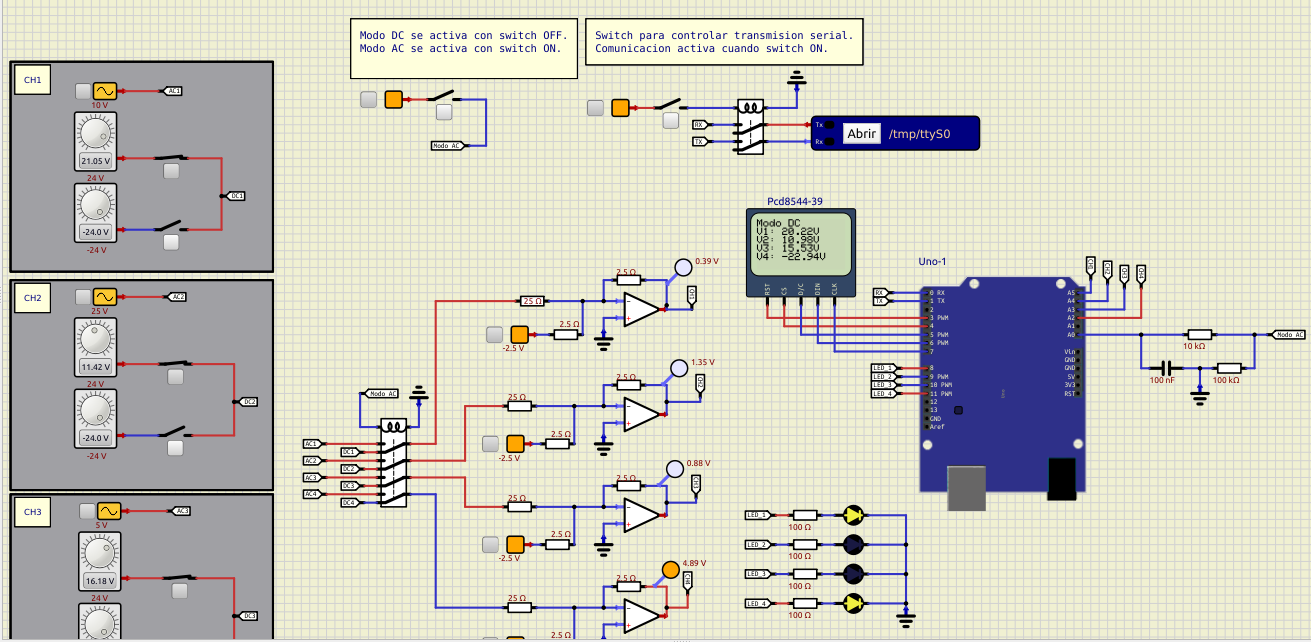
\includegraphics[width=.8\linewidth]{Imagenes/10.png}
    \caption{Activación de alarma de los LEDs.}
    \label{fig_10}
\end{figure}
Hecho esto, ahora se muestran las pruebas con tensión eléctrica en modo AC. Para realizar esta acción, se debe presionar el botón conectado al pin \texttt{A0} para ver los siguientes resultados.
\begin{figure}[H]
    \centering
    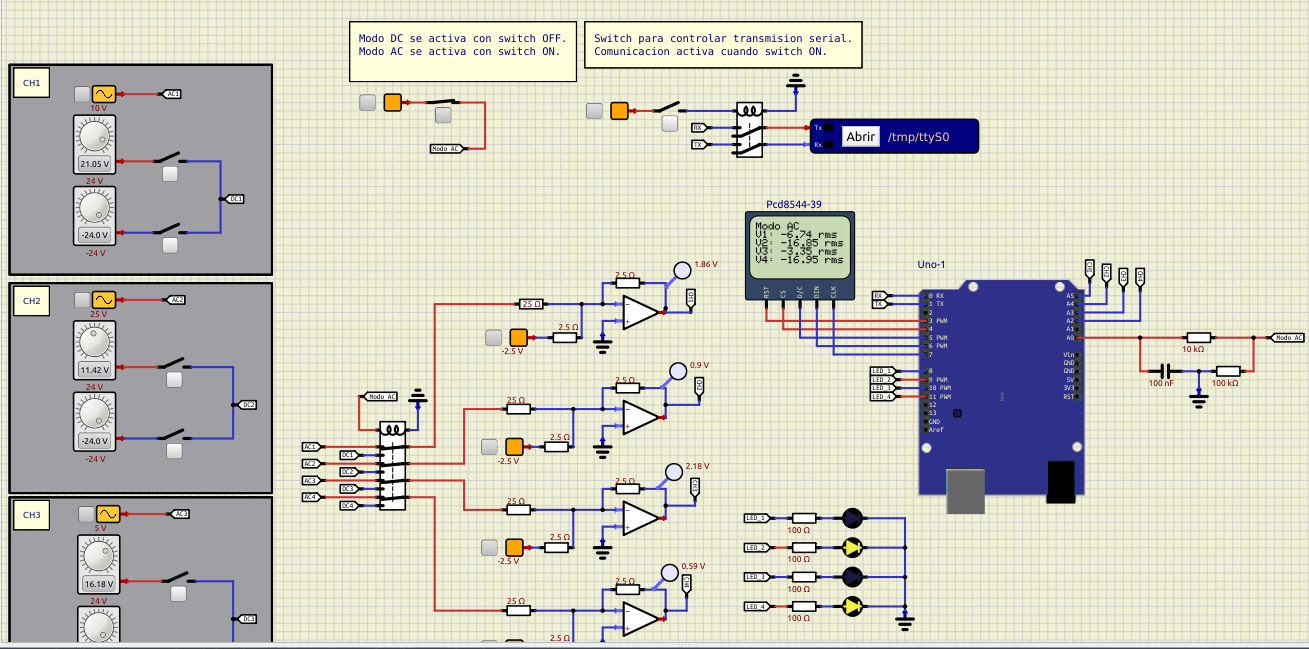
\includegraphics[width=.8\linewidth]{Imagenes/11.png}
    \caption{Medición de tensión AC de los 4 canales.}
    \label{fig_11}
\end{figure}
De la misma manera, note que en la figura \ref{fig_11} el modo AC también posee el sistema de alarmas para cuando los LEDs están fuera de los rangos permitidos: [-14.14, 14.14].\par

Para la comunicación serial se realizaron los pasos correspondientes vistos en clases, para ello primeramente se configura el script con los comando para asignar los puertos, el puerto S0 es el que realiza la comunicación con el arduino y el puerto S1 es el que se diseña para poder hacer la comunicación con el script de python y guardar los datos medidos en el archivo csv.
Primero se intentó establecer la comunicación entre el arduino y el puerto S0, de ahí que en la imagen \ref{figk1} la dirección /tmp/ttyS0, la comprobación correcta del funcionamiento se verifica en la siguiente imagen: 
\begin{figure}[H]
    \centering
    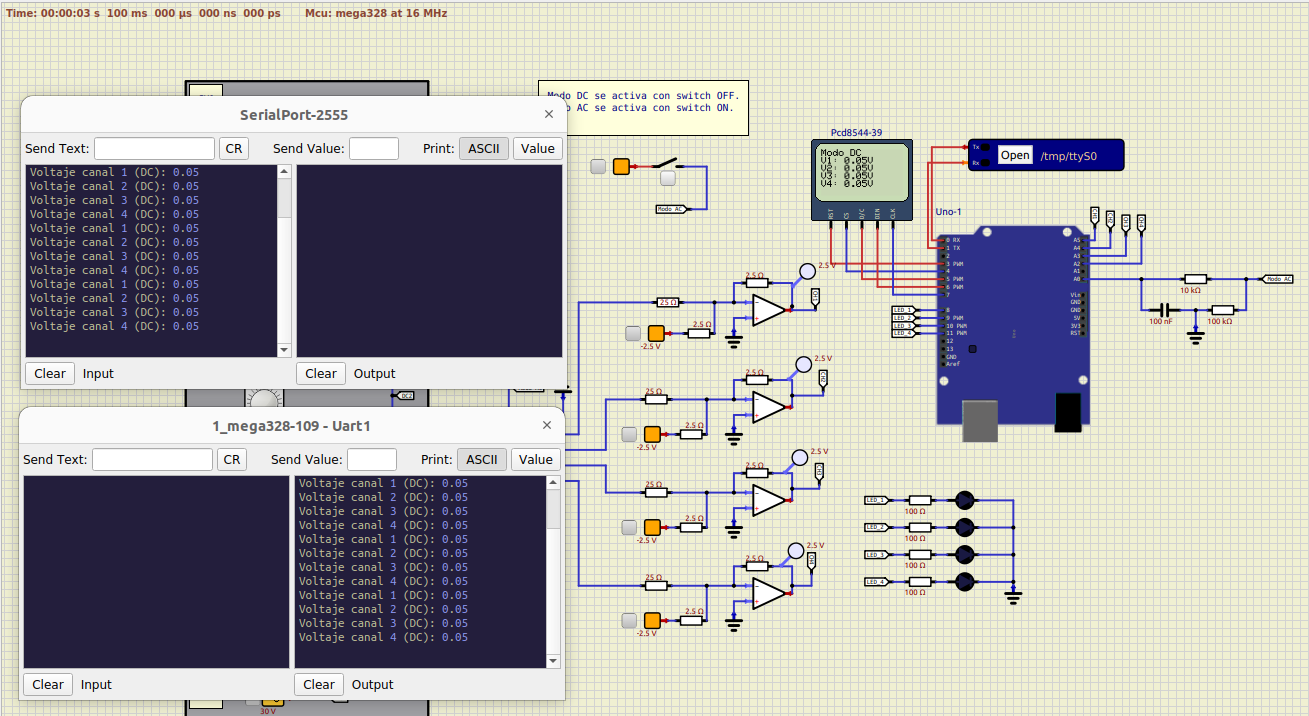
\includegraphics[width=.8\linewidth]{Imagenes/8a.png}
    \caption{Verificación de la comunicación entre el arduino y el puerto serial.}
    \label{figk2}
\end{figure}
Una vez comprobado el funcionamiento correcto de la comunicación anterior se procede a crear un puerto virtual para que pueda haber intercambio de información entre el puerto serial y el puerto serial virtual, S1, para ello se debe correr el bash script con el siguiente comando:\\
\textit{socat PTY,link=/tmp/ttyS0,raw,echo=0 PTY,link=/tmp/ttyS1,raw,echo}\\
Con este comando se crea el puerto virtual necesario, por lo que finalmente se procede a escribir un programa sencillo en python encargado de abrir un archivo csv y escribir en ello los datos correspondientes del puerto serial.\\
Los pasos para correr todo entonces es, primero correr el bash script, seguidamente abrir la comunicación en el simulador haciendo click en la opción de ''Open'', correr el script de python y finalmente correr la simulación, basado en este proceso se obtienen los siguientes resultados:
\begin{figure}[H]
    \centering
    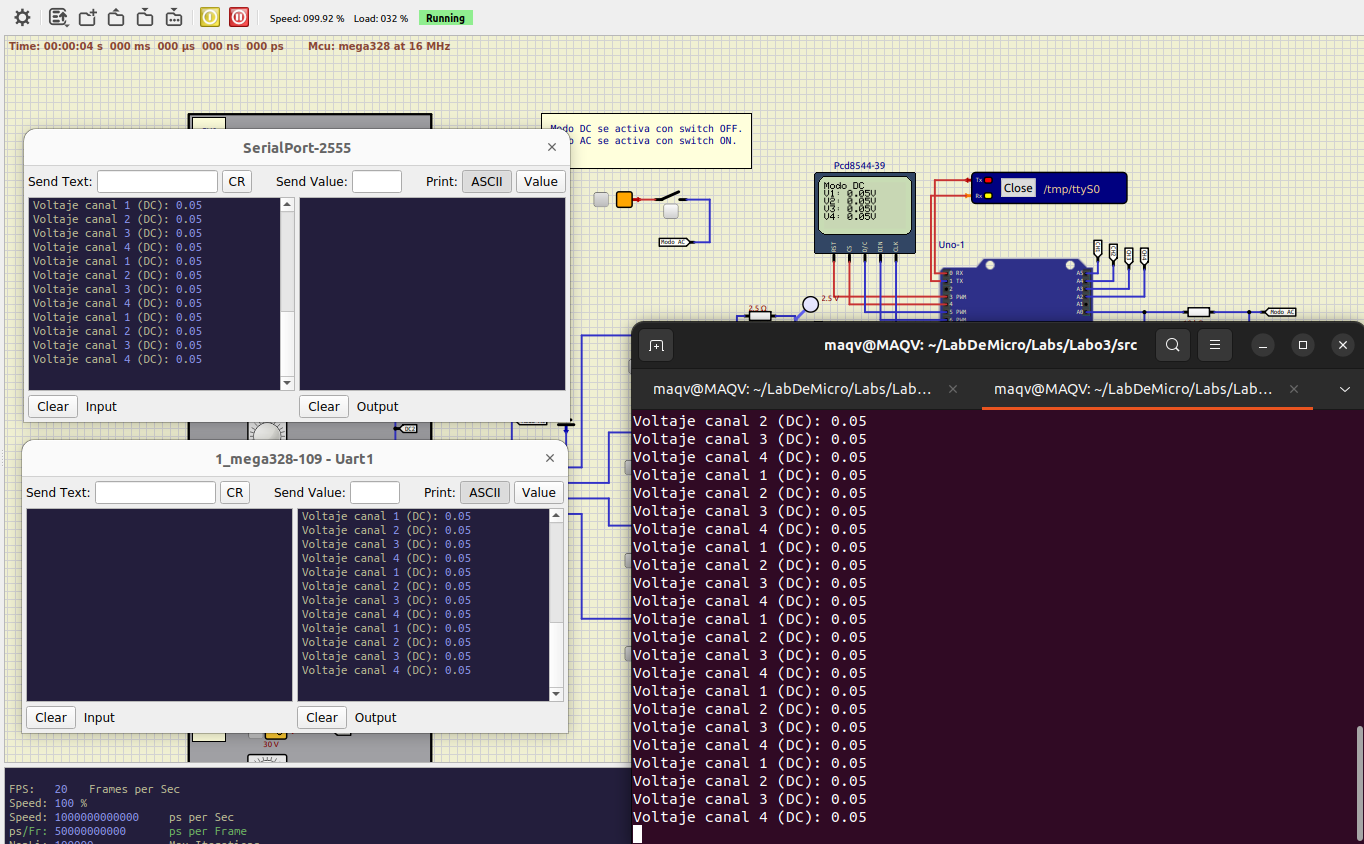
\includegraphics[width=.8\linewidth]{Imagenes/8b.png}
    \caption{Verificación de la comunicación entre el puerto serial y el puerto virtual.}
    \label{figk3}
\end{figure}
Realizando unos cambios en las fuentes de alimentación, se demuestra que por consola se obtienen los resultados esperados. Haciendo la medición en DC.
\begin{figure}[H]
    \centering
    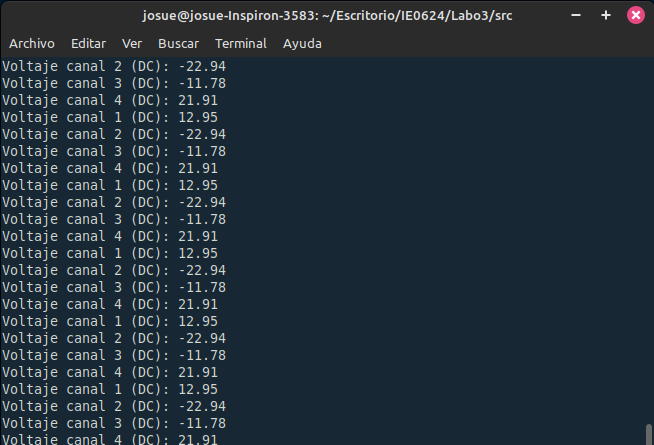
\includegraphics[width=.8\linewidth]{Imagenes/13.png}
    \caption{Medición y comunicación serial tensión DC.}
    \label{fig_13}
\end{figure}
Luego, la medición en AC.
\begin{figure}[H]
    \centering
    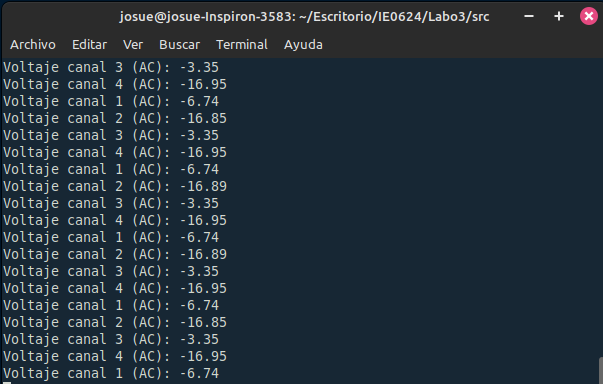
\includegraphics[width=.8\linewidth]{Imagenes/14.png}
    \caption{Medición y comunicación serial tensión AC.}
    \label{fig_14}
\end{figure}
Finalmente, se obtiene el archivo .csv generado a partir de la comunicación establecida.
\begin{figure}[H]
    \centering
    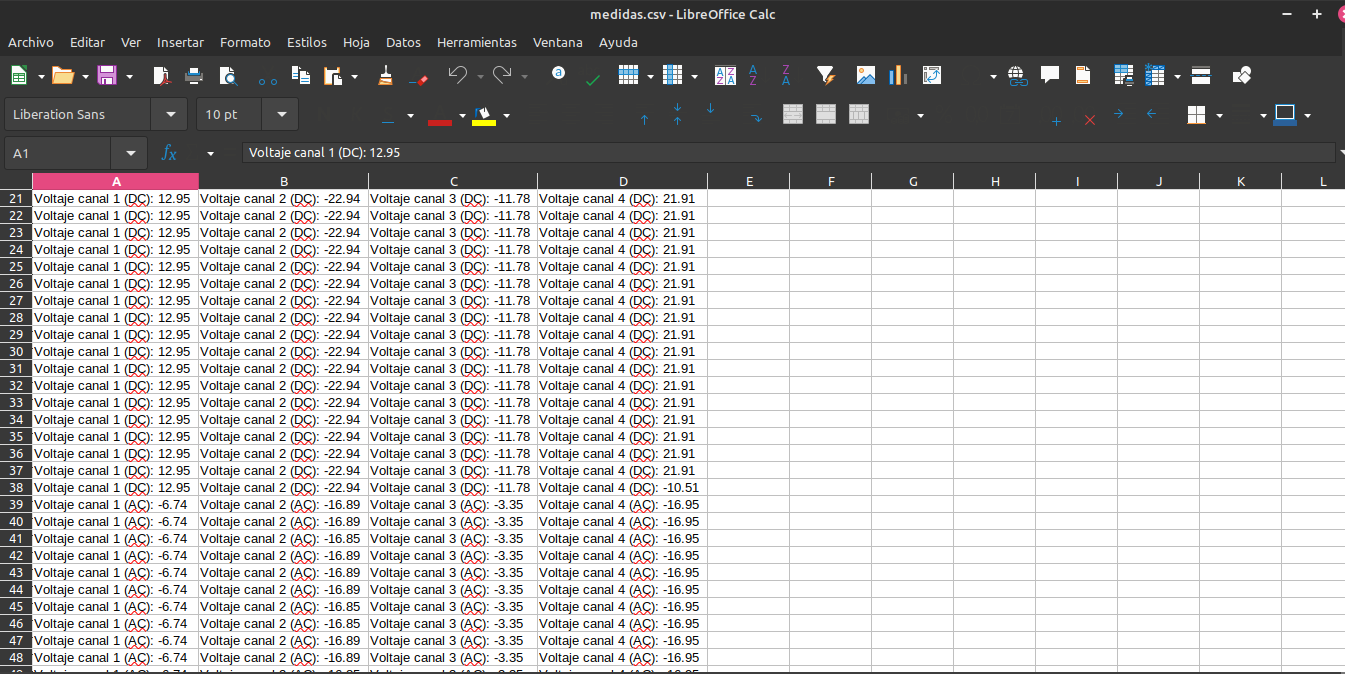
\includegraphics[width=.8\linewidth]{Imagenes/15.png}
    \caption{Archivo csv generado.}
    \label{fig_15}
\end{figure}

Ya se comprobó la generación correcta de los archivos csv, con sus respectivos valores, pero si se quisiera verificar se puede consultar el siguiente repositorio: \url{https://github.com/JosueC07183/Labo3.git} donde encontrará todos los detalles necesarios de su funcionamiento. De tal manera, que el voltímetro funciona correctamente.
\newpage
\section{Conclusiones y recomendaciones}
Para concluir,
\begin{itemize}
    \item Los puertos son de suma importancia, ya que permiten la comunicación entre otros dispositivos.
    \item Lo anterior permitió realizar el trabajo de una manera más sencilla porque las conexiones de los componentes electrónicos al mcu, así como el uso de los periféricos dieron sentido a lo que se estaba programando, desde lo más básico como la declaración de una pin como entrada o salida, como otras tareas, que suenan sencillas pero complejas si se desconoce el protocolo de comunicación de la pantalla PDC8544. 
    \item El uso de funciones ayudó a que el código se viera más ordenado, por lo que en el \texttt{loop} principal es más claro lo que está realizando. Esto es muy importante porque permitió tener un funcionamiento claro y correcto de la función del voltímetro, ya que desde las magnitudes (con cierto grado de error) asignadas en las fuentes de tensión, la normalización y el escalamiento de estos valores se mostraron correctamente en la pantalla PCD8544, y cuando se irrespetaban los umbrales de [-20,20]DC y [-14.14,14.14]AC los LEDs se encendieron, y se apagan cuando se respetaba este rango. Ahora, con respecto a la comunicación serial del arduino con la PC fue éxitosa, porque se estableció la correcta comunicación ya que lo mostrado en la pantalla se fue reflejando por consola y se guardó un archivo .csv en el directorio del proyecto. Por lo tanto, el proyecto cumple todos los requisitos solicitados.
\end{itemize}
Como recomendación se debe entender lo básico de como funciona la librería que se vaya a utilizar para poder realizar la comunicación y estar haciendo pruebas constantemente para verificar de que se esté trabajando de la forma que se espera, esto fue notable en la parte de generación del csv al igual que observar la comunicación dentro del mismo simulador porque hubieron momentos donde los datos se estaban imprimiendo de forma incorrecta.

\newpage 

\bibliographystyle{unsrt}
\bibliography{bibliografia.bib}
\newpage

  \section{Anexos}
 Aquí van las hojas del fabricante de los componentes usados para este laboratorio. 

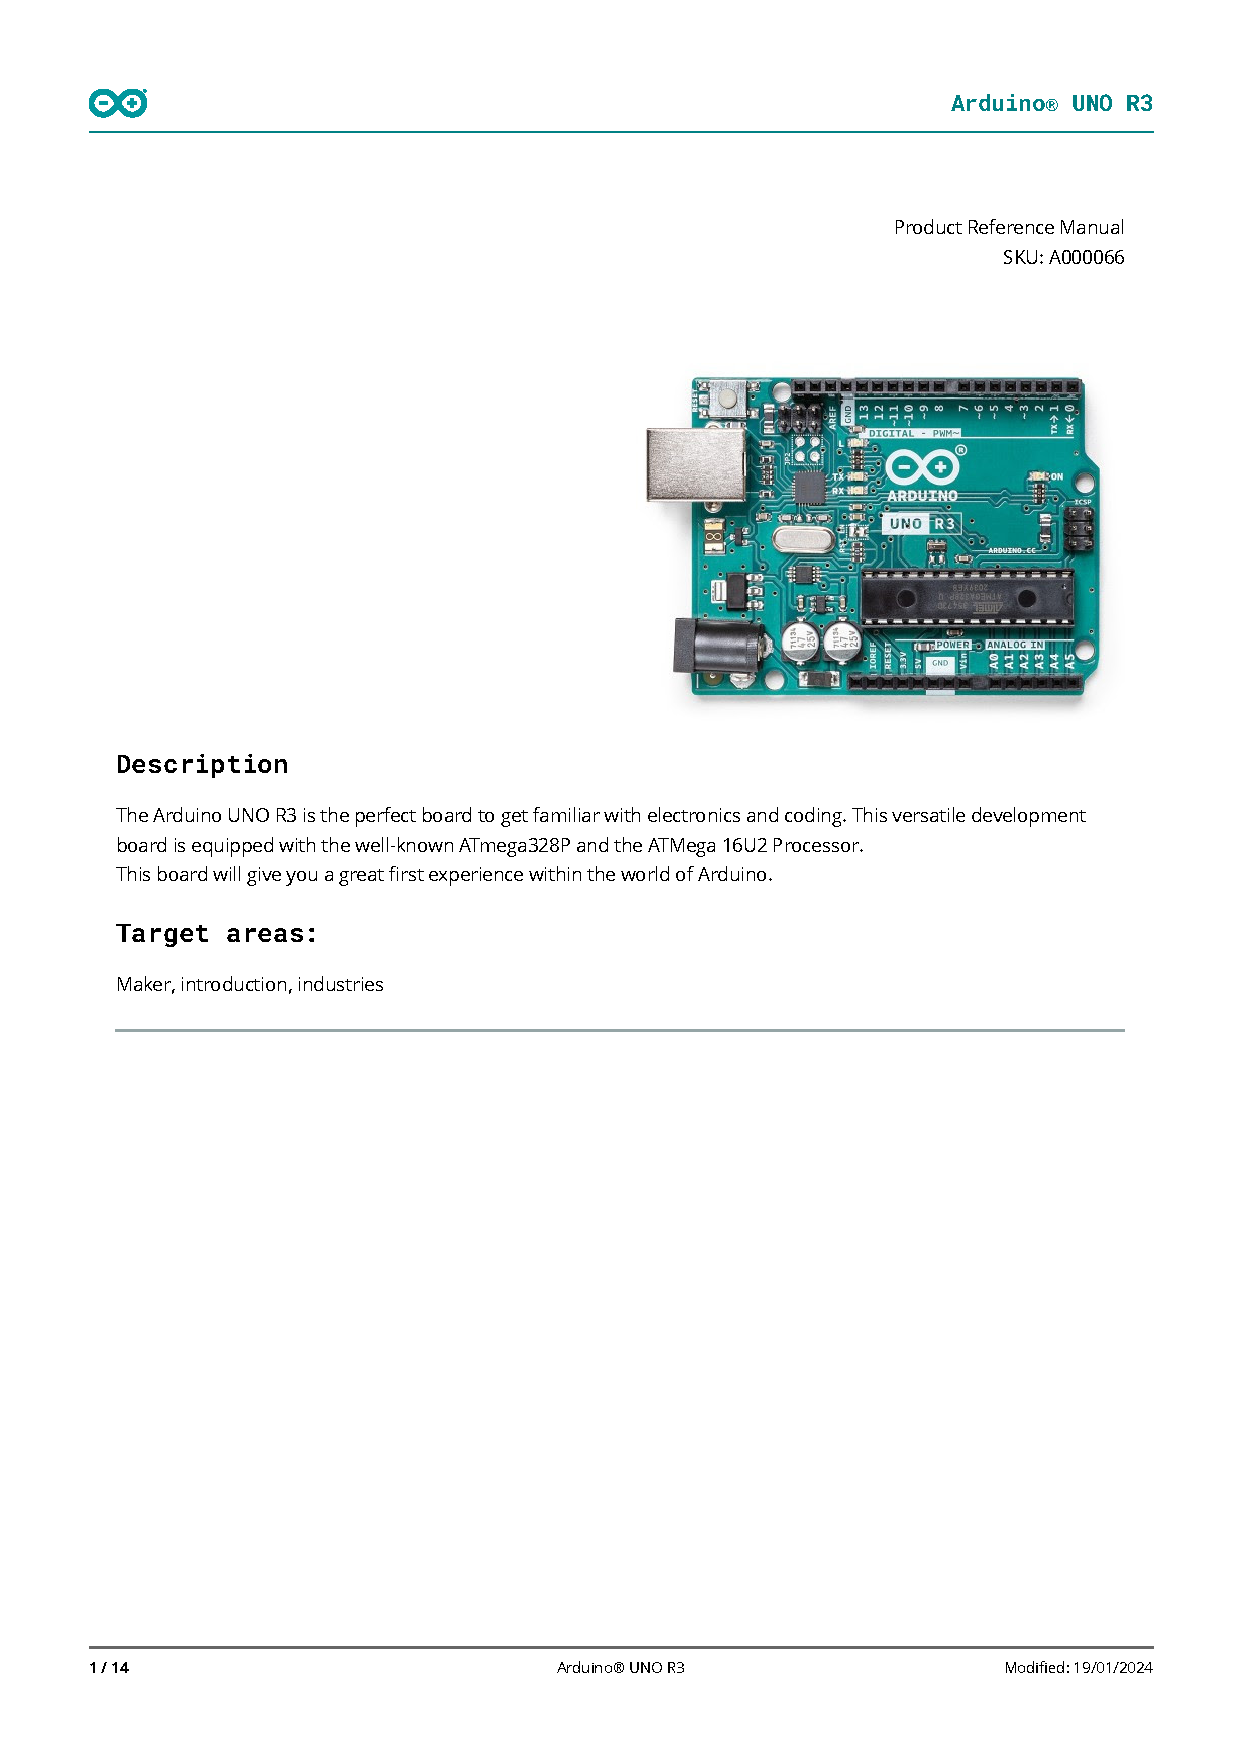
\includepdf[pages=1-14]{./Documentos/A000066-datasheet.pdf}
\foreach \page in {1,2,3,4,5,6}{
  
\includepdf[pages=\page]{./Documentos/ATMEGA48P.PDF}
}
%\foreach \page in {1,2,3}{
%  \includepdf[pages=\page]{./Documentos/cd4511b.pdf}
%}
%\foreach \page in {2,3,4}{
%  \includepdf[pages=\page]{./Documentos/display.pdf}
%}
%\includepdf[pages=1]{./Documentos/Pot.pdf}
\end{document}
 

\end{document}